% Chapter 1

\chapter{Introducción general} % Main chapter title

\label{Chapter1} % For referencing the chapter elsewhere, use \ref{Chapter1} 
\label{IntroGeneral}

%----------------------------------------------------------------------------------------

% Define some commands to keep the formatting separated from the content 
\newcommand{\keyword}[1]{\textbf{#1}}
\newcommand{\tabhead}[1]{\textbf{#1}}
\newcommand{\code}[1]{\texttt{#1}}
\newcommand{\file}[1]{\texttt{\bfseries#1}}
\newcommand{\option}[1]{\texttt{\itshape#1}}
\newcommand{\grados}{$^{\circ}$}

%----------------------------------------------------------------------------------------

En el presente capítulo se plantea el propósito de esta investigación como instrumento para dar respuesta a la necesidad latente de contar con un sistema de monitoreo remoto para la detección de incendio. Además se describe el objetivo general y los objetivos específicos que se desarrollaron; así como los alcances y las limitaciones presentadas durante el progreso de la misma.

%----------------------------------------------------------------------------------------
% \ref{fig:figura_b}
\section{Sistemas de alarmas de detección incendio}

Un elemento de gran importancia para el éxito ante situaciones de emergencia, es contar con una planificación que especifique la serie de acciones a realizar. Estos protocolos usualmente se apoyan en sistemas automatizados que brindan dos ventajas significativas: vigilancia constante de amenazas o riesgos, lo que genera un tiempo de reacción menor  y un sistema de notificación que una vez confirmada la condición de incendio notifica de manera eficiente al personal especializado y ocupantes de acuerdo a los protocolos establecidos.
El objetivo de los sistemas de detección de incendio, es reducir el impacto y las pérdidas que podrían ocasionar un incendio en el edificio o instalación a proteger. Es importante detectar una condición de incendio en el menor tiempo posible, de la manera más eficiente y segura, ya que la rápida propagación del fuego puede reducir la ventana de tiempo seguro para realizar la evacuación de las personas y disminuye el riesgo de pérdida de vidas humanas, adicionalmente estos otros beneficios que implican su instalación se pueden mencionar: proteger de bienes y servicios de la propiedad, preservar la integridad de las instalaciones, mantener la continuidad operativa del negocio, facilitar las tareas de los servicios de emergencia, además de cumplir con requerimientos específicos y regulaciones locales. En la figura \ref{fig:figura_a1} se observa un esquema con el funcionamiento básico de un sistema de detección de incendio.  

\begin{figure}[h]
	\centering
	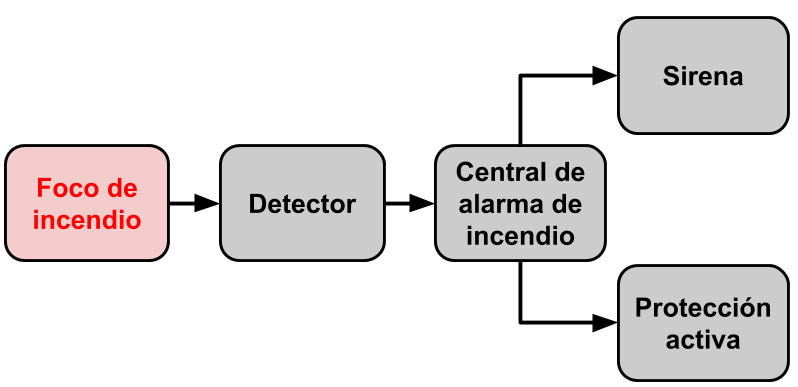
\includegraphics[scale=.4]{./Figures/Capitulo1/FIG_A1.png}
	\caption{Flujo básico de un sistema de detección de incendio.}
	\label{fig:figura_a1}
\end{figure}



\section{Sistema de notificación de alarma de incendio tradicional}

Los sistemas de alarma contra incendio se han diseñado tradicionalmente para cumplir el objetivo de detectar eventos de incendio en áreas estructurales de inmuebles que no son necesariamente monitoreados de forma constante por un personal de mantenimiento, seguridad o por los propios usuarios, lo que puede afectar el tiempo de reacción, adicionalmente se requiere que el personal asignado se encuentre correctamente instruido para la identificación de los eventos. La figura \ref{fig:figura_a2} muestra un ejemplo del flujo que se ejecuta normalmente en las instalaciones al detectarse un evento.
Estos sistemas tradicionales de detección de incendios están conformados por:

\begin{itemize}
\item Panel de control: dispositivo electrónico principal que recibe las conexiones de los diferentes artefactos que conforman al sistema, contiene toda la lógica que se debe ejecutar ante el disparo de eventos y funciona como interfaz entre el usuario y el sistema de detección de incendio.
\item Detectores: existen diferentes tipos de detectores cada uno con una tecnología particular para la detección de un riesgo específico, puede ser humo, temperatura, gases  o incluso elementos de activación manual como los pulsadores de alarma de incendio.
\item Sirenas: el aviso ante una emergencia, suele realizarse mediante el accionamiento de dispositivos de notificación sonora como sirenas o parlantes, y visual con destellos de luz estroboscópica.
\item Elementos de protección activa: ocasionalmente se puede incluir un sistema de protección más completo con subsistemas de supresión de incendio, sistemas de comunicación de emergencia, puertas cortafuego, entre otros.
\end{itemize}

\begin{figure}[h]
	\centering
	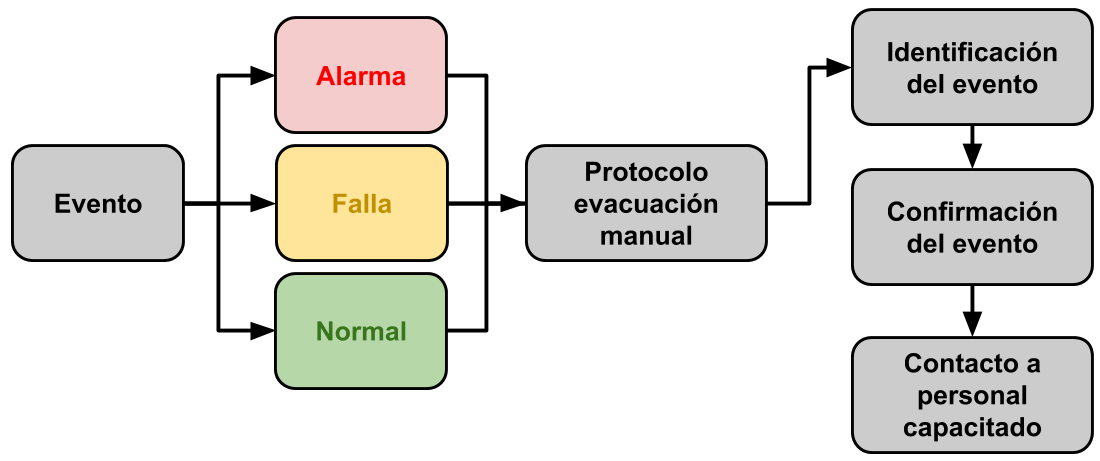
\includegraphics[scale=.35]{./Figures/Capitulo1/FIG_B1.png}
	\caption{Diagrama de ejecución de protocolos convencional ante eventos.}
	\label{fig:figura_a2}
\end{figure}

\section{Sistema de notificación de alarma de incendio propuesta}

El sistema propuesto es un equipo de monitoreo remoto de alarma de detección de incendio que indique a diferentes plataformas el estado de la instalación. El diseño evita que la comunicación de eventos entre usuarios se realice basados en la interpretación del personal que vigila la central, el sistema brinda a cada usuario  una interfaz para observar el estado de la instalación. De esta forma asegurarnos la veracidad de la información y somos capaces de notificar a todo el personal capacitado de la presencia de un evento y que no necesariamente tenga acceso al panel de control del sistema en ese instante. Las variaciones del sistema propuesto se reflejan en la figura \ref{fig:figura_a3}, donde se genera la notificación directa a diferentes entes y autoridades de la instalación.  

\begin{figure}[h]
	\centering
	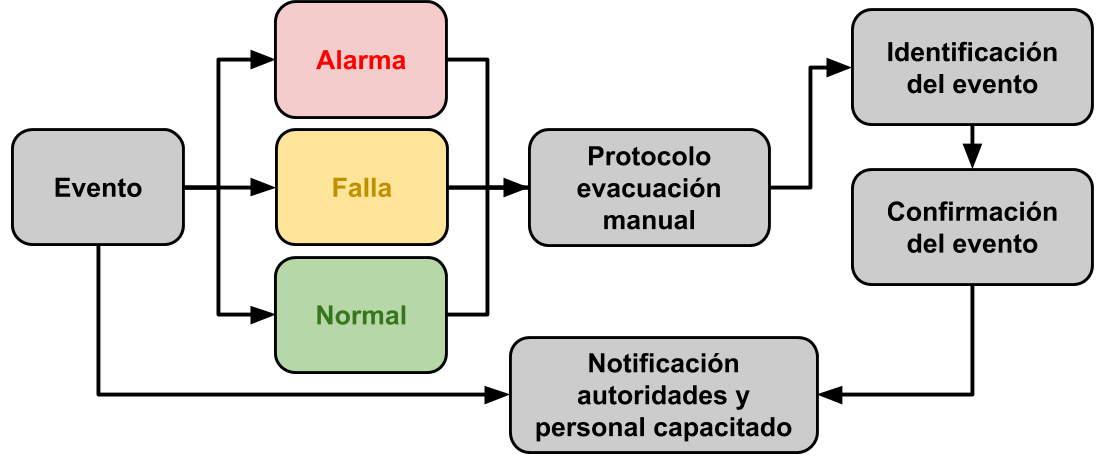
\includegraphics[scale=.35]{./Figures/Capitulo1/FIG_C1.png}
	\caption{Ejemplo de protocolo ante eventos propuesto.}
	\label{fig:figura_a3}
\end{figure}

\section{Motivación}

La firma ISOLSE SRL se dedica a la venta e instalación de sistemas de seguridad electrónica, con particular experiencia en el área de detección y supresión de incendios, cuenta con con una amplia gama de clientes repartidos en todo el territorio nacional lo cual hace necesario mantener una movilización constante de su personal técnico. 

Este proyecto surge de la necesidad detectada por la empresa ISOLSE SRL, de brindar a sus clientes y al personal técnico de ISOLSE SRL el estado del sistema de detección de incendios de las infraestructuras contratadas.

Es así como surge el planteamiento del diseño de un sistema de monitoreo de alarma de forma remota, que funcione en conjunto con las centrales de alarma de incendio, para la  inclusión de notificación de los usuarios a través de plataformas alternativas.

Este sistema brinda beneficios tanto al usuario al brindar un servicio de monitoreo constante de su instalación a través de plataformas web.  Mientras que a la empresa ISOLSE SRL el sistema diseñado le permitirá, planificar sus inspecciones de mantenimiento, o incluso coordinar visitas que antes podían ser emergencias producto de falsas alarmas, mejorando la atención al cliente y generando nuevas rutinas de prevención y mantenimiento del sistema.


\section{Estado del Arte}

A continuación se describen algunas de las opciones disponibles, estas opciones varían con respecto a las prestaciones que brindan a sus usuarios, pero todas enfocadas en complementar la notificación de eventos. 

\subsection{SafeLink}

La empresa Johnson Control desarrolló para su línea de centrales de alarmas de incendio una placa opcional que se vincula a través del protocolo de comunicación interno de la central, y genera una interfaz web con el detalle de todos los eventos que ocurren en la central. Adicionalmente al brindar conexión a Internet, el sistema tiene la capacidad de automatizar el envío de correos electrónicos a diferentes usuarios ante eventos específicos. La placa se presenta en la figura \ref{fig:figura_a3}, y es exclusiva de la marca Simplex; por lo que sus conectores varían entre cada modelo de equipo.

\begin{figure}[h]
	\centering
	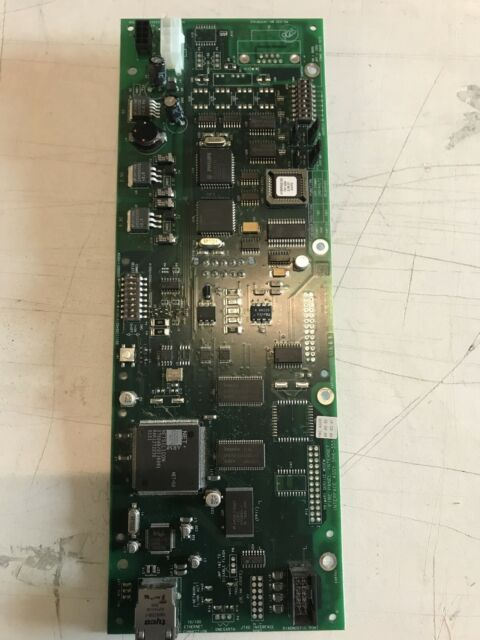
\includegraphics[scale=.4]{./Figures/Capitulo1/FIG_D1.jpg}
	\caption{Placa Safelink de Johnson Control.}
	\label{fig:figura_d1}
\end{figure}

\subsection{Haltel HT-7001}

El dispositivo corresponde al de la figura \ref{fig:figura_e1}; tiene un diseño para uso universal que permite al usuario recibir una alerta ante el disparo de una alarma. El sistema brinda la posibilidad de que el usuario visualice sus alarmas en una plataforma web, independientemente del lugar geográfico donde se encuentre. Además brinda la oportunidad de cancelar el evento si la situación así lo requiere. 

\begin{figure}[h]
	\centering
	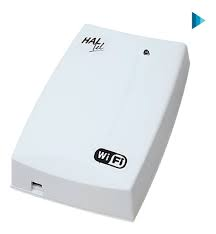
\includegraphics[scale=.4]{./Figures/Capitulo1/FIG_E1.jpeg}
	\caption{Equipo Haltel HT-7001.}
	\label{fig:figura_e1}
\end{figure}	
	
\subsection{UNO-2483G}

Corresponde a la propuesta de la empresa SPHINX, el sistema se describe en la figura \ref{fig:figura_f1}; corresponde a un sistema de detección de incendio completo, que sustituye la central de incendio por un computador de automatización embebido, la conexión con dispositivos de detección y notificación se realiza mediante dispositivos de conversión analógico digital. El sistema cuenta con una plataforma de acceso web, a través de la cual notifica cualquier evento presente.  
	
	\begin{figure}[h]
	\centering
	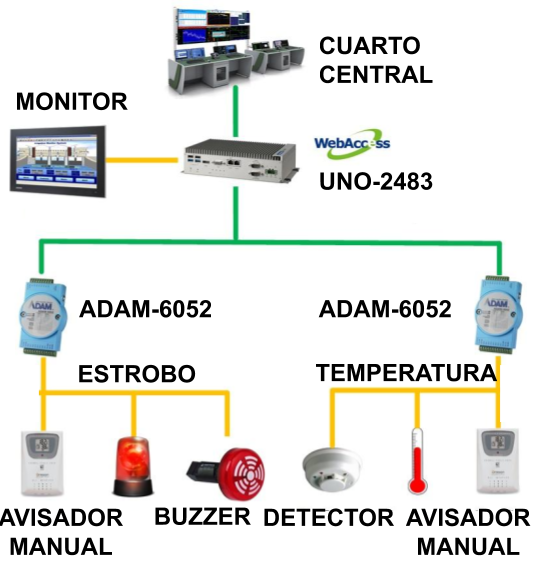
\includegraphics[scale=.4]{./Figures/Capitulo1/FIG_F1.png}
	\caption{Sistema UNO-2483G.}
	\label{fig:figura_f1}
\end{figure}

\subsection{Discador telefónico}

Son dispositivos utilizados para realizar llamadas a una lista de contactos configurable con mensajes pregrabados ante diferentes eventos de alarma, intrusión, emergencia médica, entre otros. Un ejemplo de un equipo comercial se presenta en la figura  \ref{fig:figura_g1}.  

\begin{figure}[h]
	\centering
	
\includegraphics[scale=.4]{./Figures/Capitulo1/FIG_G1.jpeg}
	\caption{Ejemplo de sistema de detección de incendio complejo.}
	\label{fig:figura_g1}
\end{figure}

\subsection{Comparativa de características}

Los sistemas descritos anteriormente se pueden analizar a través de la tabla \ref{tab:tabla_1}. Podemos observar que ninguno de los dispositivos logra reunir todas las características deseadas: un sistema con la capacidad de extraer el estado del sistema y plasmarlo en una plataforma con acceso web, que posea un tiempo de configuración corto, con compatibilidad universal para las diferentes marcas comerciales y con la posibilidad de monitorear más de un elemento dentro del sistema de detección.

\begin{table}[h]
\centering
\caption[Comparación de alternativas de estado del arte]{Comparación entre las alternativas comerciales.}
\begin{tabular}{cccccc}
\toprule
\textbf{Dispositivo}                                           & \textbf{\begin{tabular}[c]{@{}c@{}}Nivel de\\  detalle\end{tabular}} & \textbf{\begin{tabular}[c]{@{}c@{}}Acceso\\ Web\end{tabular}} & \textbf{\begin{tabular}[c]{@{}c@{}}Tiempo\\ de\\ configuración\end{tabular}} & \textbf{Marca}                                       & \textbf{\begin{tabular}[c]{@{}c@{}}Número de\\ equipos que\\ puede \\ monitorear\end{tabular}} \\
%\midrule
Safelink                                                       & Completo                                                             & Incluido                                                      & 5 horas                                                                      & Simplex                                              & 1+                                                                                             \\
%\midrule
Haltel                                                         & Básico                                                               & Incluido                                                      & 1 hora                                                                       & Universal                                            & 1                                                                                              \\
%\midrule
UNO-2483G                                                      & Completo                                                             & Incluido                                                      & +5 horas                                                                     & \begin{tabular}[c]{@{}c@{}}ADAM\\ 6052s\end{tabular} & 1+                                                                                             \\
\begin{tabular}[c]{@{}c@{}}Discador \\ telefonico\end{tabular} & Básico                                                               & \begin{tabular}[c]{@{}c@{}}No \\ Incluido\end{tabular}        & 1 hora                                                                       & Universal
			                                           & 1                                                                                             
\\
\bottomrule
\hline                                                                        
\end{tabular}
\label{tab:tabla_1}
\end{table}




\section{Alcance del proyecto}

El presente proyecto implica el diseño e implementación de un sistema de monitoreo remoto a nivel de firmware y hardware. El desarrollo se dividirá en dos componentes: el dispositivo primario y el dispositivo secundario. Se debe considerar que la comunicación entre ambos dispositivos, debe usar tecnología inalámbrica como medio de comunicación.

El sistema deberá monitorear al menos una central de alarma de incendio y hasta un máximo de 3 dispositivos secundarios, y contar con la capacidad de definir el estado de la instalación en su totalidad. Este proyecto no incluye la indicación a detalle de los eventos que ocurren en la instalación, el elemento de interés es únicamente el estado de la instalación considerando el dispositivo primario y cada uno de los dispositivos secundarios. Tampoco se considera parte del proyecto el desarrollo de interfaces de usuario, si bien se desarrollan diferentes elementos de interfaz gráfica cumplen con un objetivo de prueba de concepto más que una plataforma final.


